\documentclass{standalone}
\usepackage{tikz}
\usetikzlibrary{patterns, positioning}


\begin{document}
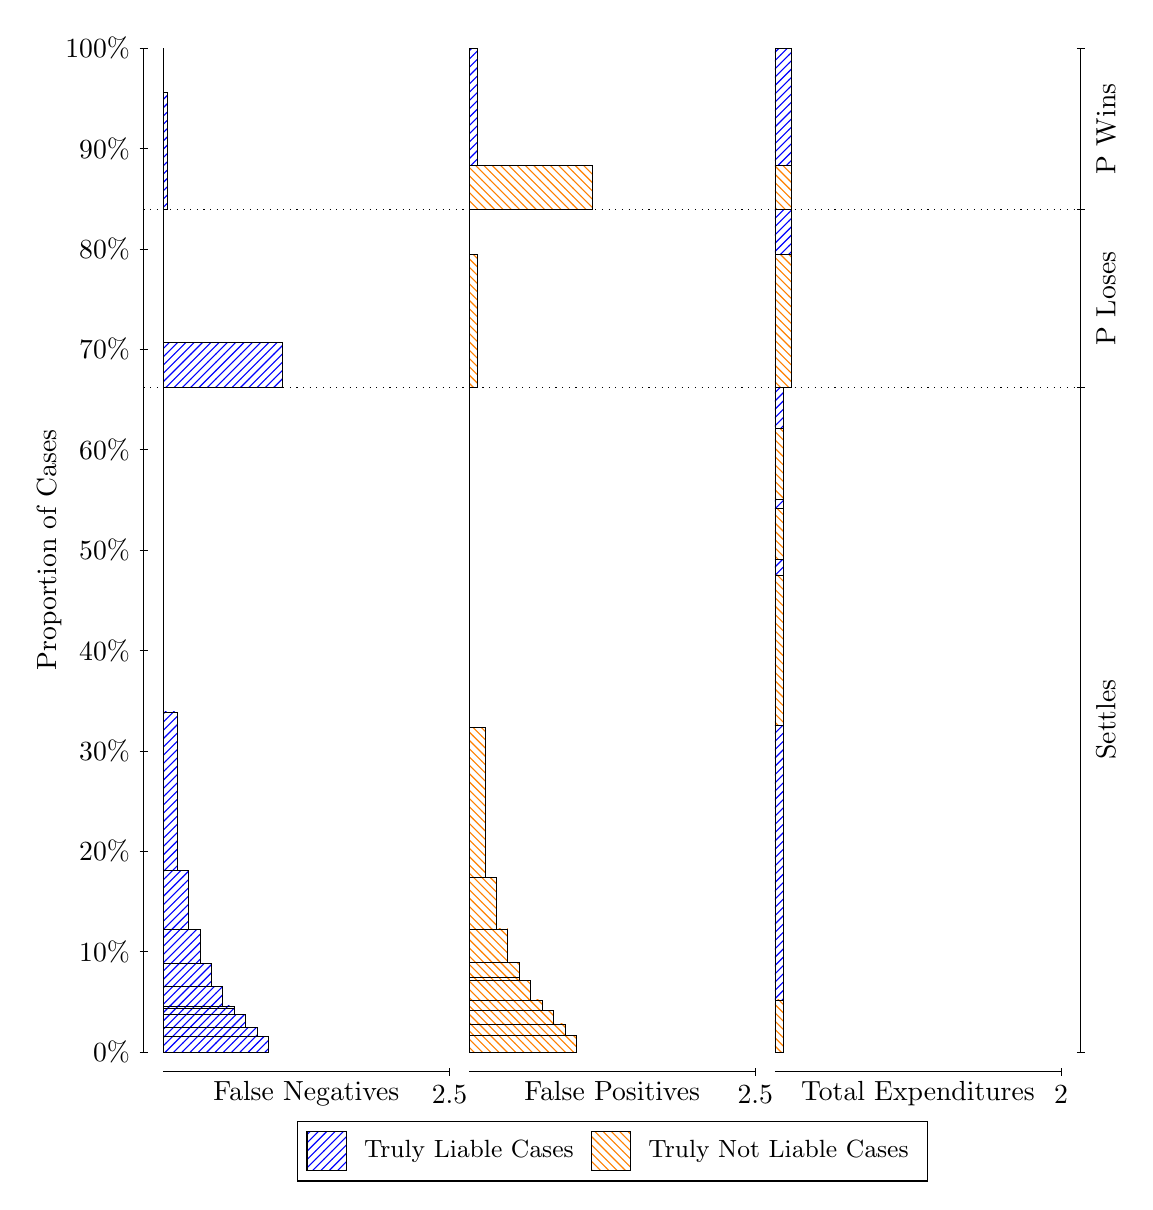
\begin{tikzpicture}
\draw[black, very thin] (1.5,1.75) -- (1.5,14.5);
\node[rotate=90, text=black, anchor=center] at (0.3, 8.125) {Proportion of Cases};
\draw[black, very thin] (1.45,1.75) -- (1.55,1.75);
\node[text=black, anchor=east] at (1.45, 1.75) {0\%};
\draw[black, very thin] (1.45,3.025) -- (1.55,3.025);
\node[text=black, anchor=east] at (1.45, 3.025) {10\%};
\draw[black, very thin] (1.45,4.3) -- (1.55,4.3);
\node[text=black, anchor=east] at (1.45, 4.3) {20\%};
\draw[black, very thin] (1.45,5.575) -- (1.55,5.575);
\node[text=black, anchor=east] at (1.45, 5.575) {30\%};
\draw[black, very thin] (1.45,6.85) -- (1.55,6.85);
\node[text=black, anchor=east] at (1.45, 6.85) {40\%};
\draw[black, very thin] (1.45,8.125) -- (1.55,8.125);
\node[text=black, anchor=east] at (1.45, 8.125) {50\%};
\draw[black, very thin] (1.45,9.4) -- (1.55,9.4);
\node[text=black, anchor=east] at (1.45, 9.4) {60\%};
\draw[black, very thin] (1.45,10.675) -- (1.55,10.675);
\node[text=black, anchor=east] at (1.45, 10.675) {70\%};
\draw[black, very thin] (1.45,11.95) -- (1.55,11.95);
\node[text=black, anchor=east] at (1.45, 11.95) {80\%};
\draw[black, very thin] (1.45,13.225) -- (1.55,13.225);
\node[text=black, anchor=east] at (1.45, 13.225) {90\%};
\draw[black, very thin] (1.45,14.5) -- (1.55,14.5);
\node[text=black, anchor=east] at (1.45, 14.5) {100\%};

\draw[black, very thin] (13.4,1.75) -- (13.4,14.5);
\draw[black, very thin] (13.35,1.75) -- (13.45,1.75);
\node[anchor=west] at (13.35, 1.75) {};
\draw[black, very thin] (13.35,10.194) -- (13.45,10.194);
\node[anchor=west] at (13.35, 10.194) {};
\draw[black, very thin] (13.35,12.446) -- (13.45,12.446);
\node[anchor=west] at (13.35, 12.446) {};
\draw[black, very thin] (13.35,14.5) -- (13.45,14.5);
\node[anchor=west] at (13.35, 14.5) {};

\draw[black, very thin, pattern color=blue, pattern=north east lines] (1.75,1.75) rectangle (3.0852,1.9483);
\draw[black, very thin, pattern color=blue, pattern=north east lines] (1.75,1.9483) rectangle (2.9399,2.0612);
\draw[black, very thin, pattern color=blue, pattern=north east lines] (1.75,2.0612) rectangle (2.7946,2.2269);
\draw[black, very thin, pattern color=blue, pattern=north east lines] (1.75,2.2269) rectangle (2.6492,2.3039);
\draw[black, very thin, pattern color=blue, pattern=north east lines] (1.75,2.3039) rectangle (2.6492,2.3348);
\draw[black, very thin, pattern color=blue, pattern=north east lines] (1.75,2.3348) rectangle (2.5039,2.5849);
\draw[black, very thin, pattern color=blue, pattern=north east lines] (1.75,2.5849) rectangle (2.3586,2.8769);
\draw[black, very thin, pattern color=blue, pattern=north east lines] (1.75,2.8769) rectangle (2.2133,3.3094);
\draw[black, very thin, pattern color=blue, pattern=north east lines] (1.75,3.3094) rectangle (2.0679,4.0515);
\draw[black, very thin, pattern color=blue, pattern=north east lines] (1.75,4.0515) rectangle (1.9226,6.0697);
\draw[black, very thin, pattern color=orange, pattern=north west lines] (1.75,6.0697) rectangle (1.75,10.194);
\draw[black, very thin, pattern color=blue, pattern=north east lines] (1.75,10.194) rectangle (3.2578,10.762);
\draw[black, very thin, pattern color=orange, pattern=north west lines] (1.75,10.762) rectangle (1.75,12.446);
\draw[black, very thin, pattern color=blue, pattern=north east lines] (1.75,12.446) rectangle (1.8045,13.932);
\draw[black, very thin, pattern color=orange, pattern=north west lines] (1.75,13.932) rectangle (1.75,14.5);
\draw[black, very thin, pattern color=orange, pattern=north west lines] (5.6333,1.75) rectangle (6.9958,1.9651);
\draw[black, very thin, pattern color=orange, pattern=north west lines] (5.6333,1.9651) rectangle (6.8505,2.1058);
\draw[black, very thin, pattern color=orange, pattern=north west lines] (5.6333,2.1058) rectangle (6.7052,2.2791);
\draw[black, very thin, pattern color=orange, pattern=north west lines] (5.6333,2.2791) rectangle (6.5598,2.4118);
\draw[black, very thin, pattern color=orange, pattern=north west lines] (5.6333,2.4118) rectangle (6.4145,2.657);
\draw[black, very thin, pattern color=orange, pattern=north west lines] (5.6333,2.657) rectangle (6.2692,2.7037);
\draw[black, very thin, pattern color=orange, pattern=north west lines] (5.6333,2.7037) rectangle (6.2692,2.8883);
\draw[black, very thin, pattern color=orange, pattern=north west lines] (5.6333,2.8883) rectangle (6.1238,3.3142);
\draw[black, very thin, pattern color=orange, pattern=north west lines] (5.6333,3.3142) rectangle (5.9785,3.963);
\draw[black, very thin, pattern color=orange, pattern=north west lines] (5.6333,3.963) rectangle (5.8332,5.874);
\draw[black, very thin, pattern color=blue, pattern=north east lines] (5.6333,5.874) rectangle (5.6333,10.194);
\draw[black, very thin, pattern color=orange, pattern=north west lines] (5.6333,10.194) rectangle (5.7423,11.877);
\draw[black, very thin, pattern color=blue, pattern=north east lines] (5.6333,11.877) rectangle (5.6333,12.446);
\draw[black, very thin, pattern color=orange, pattern=north west lines] (5.6333,12.446) rectangle (7.1957,13.013);
\draw[black, very thin, pattern color=blue, pattern=north east lines] (5.6333,13.013) rectangle (5.7423,14.5);
\draw[black, very thin, pattern color=orange, pattern=north west lines] (9.5167,1.75) rectangle (9.6189,2.4118);
\draw[black, very thin, pattern color=blue, pattern=north east lines] (9.5167,2.4118) rectangle (9.6189,5.8966);
\draw[black, very thin, pattern color=orange, pattern=north west lines] (9.5167,5.8966) rectangle (9.6189,7.8077);
\draw[black, very thin, pattern color=blue, pattern=north east lines] (9.5167,7.8077) rectangle (9.6189,8.006);
\draw[black, very thin, pattern color=orange, pattern=north west lines] (9.5167,8.006) rectangle (9.6189,8.6548);
\draw[black, very thin, pattern color=blue, pattern=north east lines] (9.5167,8.6548) rectangle (9.6189,8.7676);
\draw[black, very thin, pattern color=orange, pattern=north west lines] (9.5167,8.7676) rectangle (9.6189,9.6701);
\draw[black, very thin, pattern color=blue, pattern=north east lines] (9.5167,9.6701) rectangle (9.6189,10.194);
\draw[black, very thin, pattern color=orange, pattern=north west lines] (9.5167,10.194) rectangle (9.721,11.877);
\draw[black, very thin, pattern color=blue, pattern=north east lines] (9.5167,11.877) rectangle (9.721,12.446);
\draw[black, very thin, pattern color=orange, pattern=north west lines] (9.5167,12.446) rectangle (9.721,13.013);
\draw[black, very thin, pattern color=blue, pattern=north east lines] (9.5167,13.013) rectangle (9.721,14.5);
\draw[black, dotted] (1.5,10.194) -- (13.4,10.194);
\draw[black, dotted] (1.5,12.446) -- (13.4,12.446);
\draw[black, very thin] (1.75,1.5) -- (5.3833,1.5);
\node[text=black, anchor=north] at (3.5667, 1.5) {False Negatives};
\draw[black, very thin] (5.3833,1.45) -- (5.3833,1.55);
\node[text=black, anchor=north] at (5.3833, 1.45) {2.5};

\draw[black, very thin] (5.6333,1.5) -- (9.2667,1.5);
\node[text=black, anchor=north] at (7.45, 1.5) {False Positives};
\draw[black, very thin] (9.2667,1.45) -- (9.2667,1.55);
\node[text=black, anchor=north] at (9.2667, 1.45) {2.5};

\draw[black, very thin] (9.5167,1.5) -- (13.15,1.5);
\node[text=black, anchor=north] at (11.333, 1.5) {Total Expenditures};
\draw[black, very thin] (13.15,1.45) -- (13.15,1.55);
\node[text=black, anchor=north] at (13.15, 1.45) {2};

\node[text=black, centered, rotate=90] at (13.72, 5.9719) {Settles};
\node[text=black, centered, rotate=90] at (13.72, 11.32) {P Loses};
\node[text=black, centered, rotate=90] at (13.72, 13.473) {P Wins};

\draw (7.449999999999999,1.5) node[draw=none] (baseCoordinate) {};
\begin{scope}[align=center]
        \matrix[scale=0.5, draw=black, below=0.5cm of baseCoordinate, nodes={draw}, column sep=0.1cm]{
            \node[rectangle, draw, minimum width=0.5cm, minimum height=0.5cm, pattern color=blue, pattern=north east lines] {}; &
            \node[draw=none, font=\small, text=black] (B) {Truly Liable Cases}; &
            \node[rectangle, draw, minimum width=0.5cm, minimum height=0.5cm, pattern color=orange, pattern=north west lines] {}; &
            \node[draw=none, font=\small, text=black] (B) {Truly Not Liable Cases}; \\
            };
\end{scope}

\end{tikzpicture}
\end{document}